\documentclass[10pt,a4paper]{article}
\usepackage[utf8]{inputenc}
\usepackage[T1]{fontenc}
\usepackage{lmodern}
\usepackage[margin=1.5cm, top=1.4cm, bottom=1.4cm]{geometry}
\usepackage{hyperref}
\usepackage{enumitem}
\usepackage{titlesec}
\usepackage{xcolor}
\usepackage{graphicx}

\definecolor{accent}{HTML}{00686E}
\hypersetup{colorlinks=true, urlcolor=accent, linkcolor=accent}
\pagenumbering{arabic}
\setlength{\parindent}{0pt}

\titleformat{\section}{\large\bfseries\color{accent}}{}{0em}{}[\vspace{-0.6em}\rule{\textwidth}{0.8pt}]
\titlespacing{\section}{0pt}{7pt}{4pt}

\newcommand{\role}[4]{%
  \textbf{#1} \hfill \textbf{#2}\\[1pt]%
  \textit{#3} \hfill \textit{#4}\\[2pt]%
}
\setlist[itemize]{leftmargin=1.2em, itemsep=1.5pt, topsep=2pt, parsep=0pt}

\begin{document}

% ================= HEADER =================
\begin{minipage}[c]{0.80\textwidth}
  {\Huge\bfseries Prabhavit Gupta}\\[3pt]
  {\color{accent}\large Senior AI Product Security Engineer: Web, API \& Cloud Security}\\[6pt]
  {\footnotesize +39 351 610 7807 ~$\vert$~
  \href{mailto:prabhavitg@gmail.com}{prabhavitg@gmail.com} ~$\vert$~
  \href{https://www.linkedin.com/in/prabhavit/}{linkedin.com/in/prabhavit} ~$\vert$~
  \href{https://github.com/prab-gupta}{github.com/prab-gupta} ~$\vert$~
  Venice, Italy (CET Time Zone / EU Permanent Resident / Available Immediately)}
\end{minipage}\hfill
\begin{minipage}[c]{0.18\textwidth}
  \raggedleft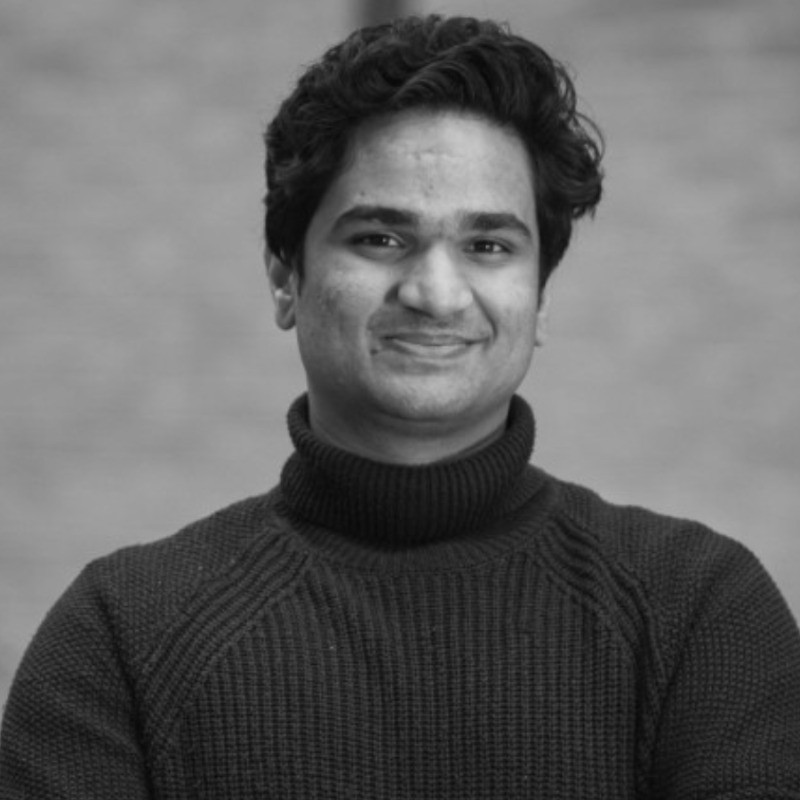
\includegraphics[width=2.0cm]{photo.jpg}
\end{minipage}
\vspace{-2pt}

% ================= SUMMARY =================
\section{Summary}
AI Product and Application Security Engineer with 3 years of production engineering experience securing enterprise AI systems, distributed microservice architectures, and cloud-native infrastructure. Proven expertise conducting rigorous Web and API security assessments, identifying OWASP Top 10 vulnerabilities, and evaluating authentication, authorization, and business logic flaws across client-facing endpoints. Skilled in container security, Kubernetes hardening, and integrating automated SAST, DAST, SCA, and secrets detection tooling directly into GitHub Actions CI/CD pipelines. Dedicated and proactive engineer available immediately for full-time remote engineering positions without notice period.

% ================= TECHNICAL EXPERTISE =================
\section{Technical Expertise}
\begin{itemize}
  \item \textbf{Product \& Application Security:} Web and REST API security testing, OWASP Top 10 / API Top 10, authentication and session management (OAuth2, OIDC, JWT), RBAC/ABAC authorization testing, threat modeling, business logic abuse prevention.
  \item \textbf{Security Testing \& Tooling:} Burp Suite, OWASP ZAP, vulnerability discovery and validation, SAST/DAST tooling, dependency scanning (Trivy, Dependabot), automated secret scanning (TruffleHog, Gitleaks).
  \item \textbf{Cloud \& Container Security:} Kubernetes pod security standards, container image hardening (distroless/minimal base images), cloud IAM least-privilege policies, secret management, ingress TLS configuration.
  \item \textbf{Secure SDLC \& CI/CD:} Automated security gates in GitHub Actions, PR quality gates, regression test automation with pytest and Playwright, code review security practices.
  \item \textbf{Languages \& Backend:} Python (FastAPI, asyncio, requests), TypeScript/Node.js, SQL (PostgreSQL, query hardening, SQL injection prevention), Bash shell scripting.
  \item \textbf{Languages \& Availability:} English (C1 Professional, fluent), Hindi (Native), Italian (Conversational). Available immediately without notice period.
\end{itemize}

% ================= EXPERIENCE =================
\section{Experience}

\role{\href{https://flowspace.co}{FlowSpace.co}}{Mar 2024 - Aug 2026}{Lead AI Application \& Security Engineer}{London, UK (remote)}
\begin{itemize}
  \item Led security assessments across enterprise AI products and API services, auditing 15+ external API connectors and client-facing endpoints serving 4,500+ users.
  \item Performed hands-on vulnerability testing using Burp Suite and OWASP ZAP, identifying and remediating authorization bypasses, SSRF risks, and token handling bugs.
  \item Integrated automated SAST, dependency vulnerability scanning (Trivy), and secret scanning gates into GitHub Actions CI/CD pipelines, blocking insecure commits prior to deployment.
  \item Hardened Docker container build pipelines and Kubernetes cluster manifests, enforcing non-root users, read-only root filesystems, and minimal network attack surfaces.
  \item Authored threat models and risk assessment matrices for autonomous agentic workflows and tool-calling integrations, preventing indirect prompt injection exploits.
\end{itemize}

\role{Urlink}{Apr 2025 - Jul 2025}{Application Security \& Platform Developer (Freelance)}{Barcelona, Spain (remote)}
\begin{itemize}
  \item Conducted security testing of external REST API endpoints, implementing automated payload sanitization, strict Pydantic schema validation, and rate-limiting controls.
  \item Configured automated security regression test suites with pytest and Playwright, testing session invalidation, CORS configurations, and TLS enforcement.
  \item Audited cloud infrastructure configurations and Docker environments to ensure secure credential isolation and minimal attack surface exposure.
\end{itemize}

\role{Independent Technical Consultant}{Aug 2023 - Feb 2024}{Security \& Systems Engineer}{Venice, Italy}
\begin{itemize}
  \item Performed application security assessments and code reviews for European SMB web applications, hardening authentication flows and database queries.
  \item Deployed automated vulnerability scanners and log auditing scripts on Linux servers, providing actionable remediation reports to development teams.
  \item Authored secure coding standards and API integration guidelines for client developers.
\end{itemize}

% ================= EDUCATION =================
\section{Education}
\role{Ca' Foscari University of Venice}{2020 - 2024}{BA in Philosophy, International Studies and Economics}{Venice, Italy}
\begin{itemize}
  \item Rigorous training in formal logic, statistical inference, quantitative economics, and complex systems modeling.
\end{itemize}

\end{document}
